\section{Introduction}
\label{sec:introduction}
On-device processing is emerging as a vital component of modern human detection and tracking systems, particularly as a strategy to enhance privacy and data security. The ability to detect and track humans in real-time is essential across a range of applications, from security surveillance to visitor analytics in cultural institutions. However, the deployment of these systems, especially in sensitive environments like museums and aquariums, raises significant privacy and data security concerns. This thesis explores the development and deployment of a privacy-preserving human localization system, specifically addressing the challenges posed by on-device processing where images are deleted post-inference. This process complicates the validation of inference accuracy, especially since many models trained on large, generic datasets may not perform equivalently in specific deployment scenarios.

\subsection{Background and Motivation}
The method of human detection and tracking in public spaces has significantly evolved over the past decade, driven by advancements in computer vision and machine learning. Traditional surveillance systems typically relied on centralized processing, where video feeds were transmitted to a remote server for analysis. This approach not only raised privacy concerns due to the potential exposure of sensitive information but also required substantial human intervention, making it time-consuming, error-prone, and lacking in scalability. This thesis advocates for a shift towards \textit{on-device} processing, which performs analytics locally on the edge device, thereby eliminating the need to transmit raw video data and significantly enhancing privacy. This is particularly relevant for environments such as museums and aquariums where privacy preservation is critical.

To demonstrate the feasibility and effectiveness of on-device human detection and localization in a practical setting, two devices were deployed in the "Fiskeri og Søfartsmuseet" aquarium in Esbjerg, Denmark. The deployment aimed to address the unique challenges of indoor, low-light environments. A dataset of 3397 images was collected and labeled, and was used to evaluate and fine-tune several object detector machine learning models. The best performing model was subsequently deployed to collect anonymous data on visitors over a month, with results visualized through heatmaps and analysis of peak visitation hours.

\newpage
\subsection{Scope}
The scope of this project is dualistic. It encompasses demonstrating a comprehensive implementation of a privacy-preserving human localization system. It also encompasses critically assessing the validity of object detection model performances across general and specific datasets to understand the real-world impacts of scientific advancements.

The project spanned several disciplines and required research, development, and effort in edge-device deployment, machine learning, and data science. Choices were made to focus the scope to manage the workload effectively.

\paragraph{Secure Control of Device}
\phantomsection
\label{sec:scope_ssh}
A dataset was built of consenting individuals in an aquarium which was part of a larger museum facility. However, once development was finished and the system was tested, the devices were actively photographing individuals who had \textit{not} given consent to be photographed. Privacy was still preserved by immediately inferencing on and deleting the images. In such an application, it is imperative to not store or upload clear, privacy-intrusive images. Therefore, an existing and already proven secure solution developed by \textit{HallMonitor}, a company specializing in on-device processing solutions based in Esbjerg, was utilized to establish a secure communication channel with the deployed devices. The communication channel was used to extract the analytics data from the devices. This secure system setup, necessary to protect the devices from attackers, is not covered in this thesis due to its proprietary nature.

\paragraph{Fine-tuned Model Development}
The project's broad scope resulted in a limited exploration of potential improvements in model fine-tuning. This thesis evaluates the performance of various machine learning models, including models built from the three arhitectures YOLOv3, YOLOv9, and DETR. Two more object detection architectures are also mentioned, but were not (fully) implemented. These are Co-DETR, the current best-performing model on the COCO dataset, and the Faster-RCNN, another popular and good option for object detection. However, the Co-DETR was deemed too complex and resource-intensive for the project's scope to be fully implemented and evaluated, and Faster-RCNN was not prioritized due to it performing worse than the YOLOv9 in multiple experiments. The object detectors are discussed in section \ref{sec:object_detection}.

\paragraph{Museum and Aquarium Opening Hours and Visitor Conduct}
\phantomsection
\label{sec:scope_opening_hours}
The project was to not interfere with the normal operations of the aquarium. This meant the only hours to capture images for the dataset was within opening hours, and it meant not asking random visitors if they would be willing to participate in the project. By an early analysis of the visitation patterns, most visitors were there early in the morning from the opening at 10:00, until around 2 hours before closing time 17:00. This was the opportunity window for getting images collected for the dataset.

\paragraph{Task is Object Detection}
\phantomsection
\label{sec:scope_object_detection}
There are several tasks within the domain of computer vision, each serving distinct purposes and complexities. This project focuses exclusively on simple object detection, which involves locating objects of relevance within an image. Specifically, this thesis addresses single-class object detection with \textit{person} as the sole class of interest. Other tasks in computer vision include person re-identification, image classification, combined image classification and localization, semantic segmentation, and instance segmentation. Re-identification involves recognizing individuals across different images and image classification is the task of classifying the image contents as a whole. The rest of the tasks are illustrated in figure \ref{fig:computer_vision_tasks} to display how they differentiate from object detection. 

\begin{figure}[H]
    \centering
    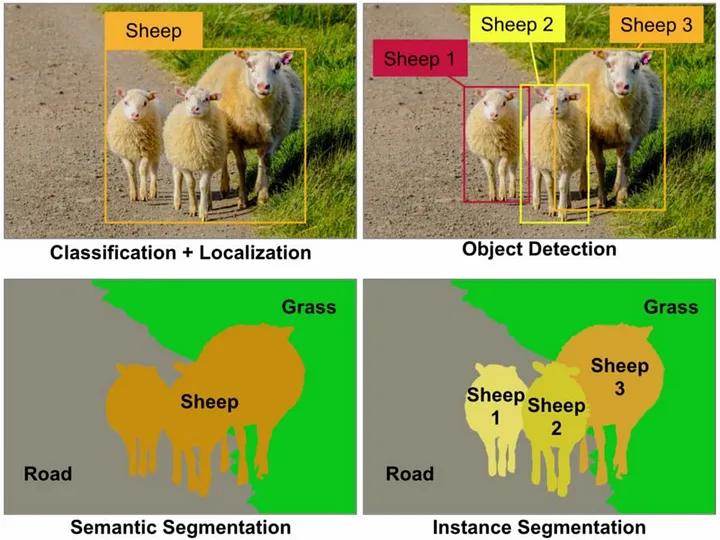
\includegraphics[width=0.6\linewidth]{Images/computer_vision_tasks.png}
    \caption{Image processing tasks (\cite{mu2021object_detection_operations}).}
    \label{fig:computer_vision_tasks}
\end{figure}

The selection of a dataset must be directly aligned with the specific task to be performed, as it must contain data suited for that task. For instance, applications tasked with person reidentification require a dataset that includes the identities across images for the persons depicted in the images. An appropriate dataset for such applications, the Person Reidentification in the Wild (PRW), is detailed in section \ref{sec:dataset_PRW}.

\paragraph{TinyML and Frugal Devices}
\phantomsection
\label{sec:scope_tinyML}
An initial attempt was made to encompass tinyML and frugal devices in the project. This, however, was scoped out of the thesis. 

\subsubsection{Research Questions}
\label{sec:research_questions}
The following research questions are meant to guide the focus of this thesis.
\begin{enumerate}
	\item What are some privacy risks associated with traditional human localization systems in public spaces, and how may on-device processing mitigate these privacy concerns?
	\item How does the validity of object detection model evaluations change when using data specifically from the intended deployment environment compared to using generic datasets?
	\item What are some machine learning architectures suitable for object detection in a real-world deployment scenario?
\end{enumerate}

\subsubsection{Research Objectives}
\label{sec:research_objectives}
\paragraph{The Primary Objectives are to:}
\begin{enumerate}
	\item Develop a privacy-preserving human localization system using on-device processing to minimize data transmission and enhance data privacy.
	\item Demonstrate feasability and effectiveness of on-device human detection and tracking in a practical and realistic setting.
	\item Investigate the effects of the dataset quality in fine-tuning of models on the performance.
	\item Assess the impact of deployment-specific data on the accuracy and validity of object detection model evaluations, by comparing performance metrics with those obtained using generic datasets.
\end{enumerate}

\paragraph{The Secondary Objectives are to:}
\begin{enumerate}
	\item Compare the privacy and performance impacts of on-device processing against traditional centralized methods.
	\item Investigate the feasibility of deploying the developed system in other public spaces to enhance visitor analytics and security.
	\item Demonstate how to visualize object detection data by creating visualizations of collected data from a realistic setting.
	\item Explore relevant object detection architectures to evaluate their performance in a real-world deployment sceneario.
\end{enumerate}
% todo sammenligne dataen de har på hvor mange besøkende på en dag. Har de data om når på dagen det er travlest? Vet du hvor mange som er i innom akvariet?


\subsection{Structure}
\label{sec:structure}
The thesis is structured as follows:

\textbf{Section \ref{sec:literature}: Literature Review} - Surveys existing technologies and discusses the theoretical underpinnings of the project.

\textbf{Section \ref{sec:methodology}: Methodology} - Details the technical methods and materials used in the project.

\textbf{Section \ref{sec:results}: Results and Discussion} - Analyzes the data collected, evaluates the system's performance, and discusses the findings.

\textbf{Section \ref{sec:conclusions}: Conclusions and Future Work} - Summarizes the research contributions and outlines potential future research directions.
